\documentclass[tikz,border=2pt]{standalone}
\usepackage{amsmath,amssymb}
\usepackage{tikz}

\begin{document}
% Choosing 2 letters out of {A,B,C,D} without regard to order: the 12 ordered pairs collapse
% in twos to the 6 combinations, C(4,2) = 4*3/2! = 6.
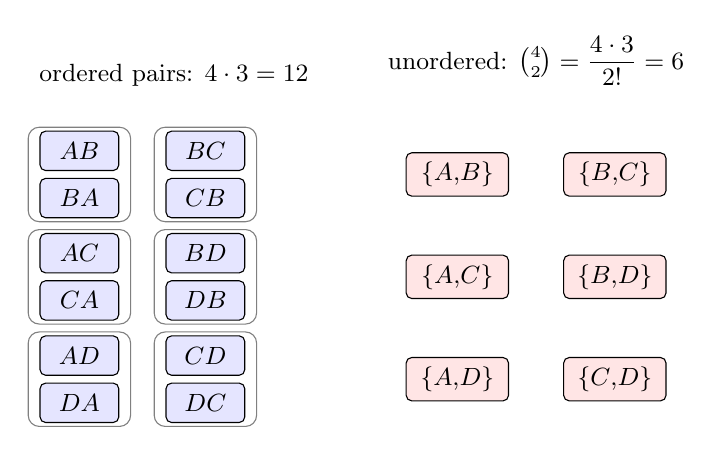
\begin{tikzpicture}[every node/.style={font=\small}]
	\node[anchor=south] at (0,1.9) {ordered pairs: $4\cdot3=12$};
	\foreach \p/\x/\y in {AB/-1.2/1.2, BA/-1.2/0.6, AC/-1.2/-0.1, CA/-1.2/-0.7, AD/-1.2/-1.4, DA/-1.2/-2.0, BC/0.4/1.2, CB/0.4/0.6, BD/0.4/-0.1, DB/0.4/-0.7, CD/0.4/-1.4, DC/0.4/-2.0} {
		\node[draw, fill=blue!10, rounded corners=2pt, minimum width=1cm, minimum height=5mm] at (\x,\y) {$\p$};
	}
	\foreach \y in {0.9,-0.4,-1.7} {\draw[gray, rounded corners=4pt] (-1.85,\y+0.6) rectangle (-0.55,\y-0.6); \draw[gray, rounded corners=4pt] (-0.25,\y+0.6) rectangle (1.05,\y-0.6);}
	\node[anchor=south] at (4.6,1.9) {unordered: $\binom42=\dfrac{4\cdot3}{2!}=6$};
	\foreach \p/\y in {\{A{,}B\}/0.9, \{A{,}C\}/-0.4, \{A{,}D\}/-1.7} {\node[draw, fill=red!10, rounded corners=2pt, minimum width=1.3cm, minimum height=5mm] at (3.6,\y) {$\p$};}
	\foreach \p/\y in {\{B{,}C\}/0.9, \{B{,}D\}/-0.4, \{C{,}D\}/-1.7} {\node[draw, fill=red!10, rounded corners=2pt, minimum width=1.3cm, minimum height=5mm] at (5.6,\y) {$\p$};}
	
\end{tikzpicture}
\end{document}
